\chapter{Appendix}

%------------------------------------------------------------------------------

\section{Payload Configurations}
\label{sec:pyldConfigs}
\begin{table}[H]
	\caption{UAV sensor payload configuration}
	\centering
	\rowcolors{1}{lightgray}{white}
	\label{tab:uavSensorMap}
	\begin{tabular}{|p{1cm}|p{1cm}|p{1cm}|}
		\hline
		UAV Type & Sensor Type\\ \hline
		0 & 0 \\
		1 & 1 \\
		\hline
	\end{tabular}
\end{table}

\begin{table}[H]
	\caption{UAV weapon payload configuration}
	\centering
	\rowcolors{1}{lightgray}{white}
	\label{tab:uavWpnMap}
	\begin{tabular}{|p{1cm}|p{1.5cm}|p{2cm}|}
		\hline
		UAV Type & Weapon Type & Initial Quantity\\ \hline
		1 & 0 & 4 \\
		1 & 1 & 4 \\
		\hline
	\end{tabular}
\end{table}

%------------------------------------------------------------------------------

\section{Algorithms}
\label{sec:algorithms}

\begin{algorithm}[H]
	\caption{UAV Foraging - Selecting a cell to search}
	\label{alg:forage}
	\begin{algorithmic}[1]
		\Function{GenerateForageLocation}{}
			\Require $ 0\le randomWeighting \le 1$
			\Require $ kernelSize \ll min($number world rows, number world columns$)$
			\Require $ \frac{number world rows}{kernelSize} \in Z$
			\Require $ \frac{number world columns}{kernelSize} \in Z$
			\Ensure $ 0 \le x \le $ number world rows
			\Ensure $ 0 \le y \le $ number world columns
			\State $rowsPerKernel\gets $ number world rows $ / kernelSize$
			\State $colsPerKernel\gets $ number world columns $ / kernelSize$		
			\State $x\gets -1$
			\State $y\gets -1$
			\State $maxUncertainty\gets -1$
			\State $maxUncertRow\gets -1$
			\State $maxUncertCol\gets -1$
			
			
			\If{$random() < randomWeighting$}
				\State $ y\gets $ random row
				\State $ x\gets $ random column
			\Else
				\For{$i\gets0$, $i < $number world rows, $i\gets i + rowsPerKernel$}
					\For{$j\gets0$, $j <$ number world columns, $j\gets j + colsPerKernel$}
						\State $kernelUncert\gets computeKernelUncert(i,j, kernelSize)$
						\If{$kernelUncert > maxUncertainty$}
							\State $maxUncertainty\gets kernelUncert$
							\State $maxUncertRow\gets i$
							\State $maxUncertCol\gets j$	
						\EndIf
					\EndFor
				\EndFor
				\State $x\gets randomInteger(rowPerKernel) + maxUncertRow$			
				\State $y\gets randomInteger(colsPerKernel) + maxUncertCol$
			\EndIf \\
			
			\Return x, y
		\EndFunction
	\end{algorithmic}
\end{algorithm}

\begin{algorithm}[H]
	\caption{Cell Belief Merging}
	\label{alg:mergeCell}
	\begin{algorithmic}[1]
		\Function{MergeCells}{$myCells[][], otherCells[][]$}
		\State $numRows\gets $ number of world rows
		\State $numCols\gets $ number of world columns
		\State $alpha\gets $ user defined weighting value in [0,1]
		\For{$i\gets 0, numRows$}
			\For{$j\gets 0, numCols$}
				\If{$otherCells_{ij}.lastUpdateTime > myCells_{ij}.lastUpdateTime$}
					\State $myCells_{ij}.probCellEmpty\gets alpha * otherCells_{ij}.probCellEmpty + (1-alpha) * myCells_{ij}.probCellEmpty$
					\State $myCells_{ij}.lastUpdateTime\gets otherCells_{ij}.lastUpdateTime$
				\EndIf
			\EndFor
		\EndFor
		\EndFunction
	\end{algorithmic}
\end{algorithm}

\begin{algorithm}[H]
	\caption{Target Belief Merging}
	\label{alg:mergeTarget}
	\begin{algorithmic}[1]
		\Function{MergeTargets}{$myTarget, otherTarget$}
		\State $alpha\gets $ user defined weighting value
		\If{$otherTarget.lastUpdateTime > myTarget.lastUpdateTime$}
			\State $myTarget.heading\gets alpha * otherTarget.heading + (1-alpha)*myTarget.heading$
			\State \Call{InterpolateCoordinate}{$myTarget.location, otherTarget.location, alpha$}
			\For{$i\gets 0, $ number of target types}
				\State $myTarget.probTypes[i]\gets alpha * otherTarget.probTypes[i] + (1-alpha)*myTarget.probTypes[i]$
			\EndFor
			\State $myTarget.lastUpdateTime\gets otherTarget.lastUpdateTime$
		\EndIf
		\EndFunction
		\\
		\Function{InterpolateCoordinate}{from, to, percentage}
			\State $deltaNorth\gets to.north - from.north$
			\State $deltaEast\gets to.east - from.east$
			\State $from.north\gets from.north + deltaNorth * percentage$
			\State $from.east\gets from.east + deltaEast * percentage$
		\EndFunction
	\end{algorithmic}
\end{algorithm}

\begin{algorithm}[H]
	\caption{Target Task Status Merging}
	\label{alg:mergeTaskStatus}
	\begin{algorithmic}[1]
		\Function{MergeTargetTaskStatus}{$myTask, otherTask$}
		\State $copyMonitorData\gets false$
		\State $copyAttackData\gets false$
		\\
		\If{$otherTask.monitorState == Complete and myTask.monitorState != otherTask.monitorState$}
			\State $copyMonitorData\gets true$
			\Comment Another UAV completed the task
		\ElsIf{$otherTask.monitorScore > myTask.monitorScore and otherTask.monitorState != Complete and myTask.monitorState != Complete$}
			\State $copyMonitorData\gets true$
			\Comment Everyone is bidding on the task still
		\EndIf
		\\
		\If{$copyMonitorData == true$}
			\State $myTask.monitorID\gets otherTask.monitorID$
			\State $myTask.monitorScore\gets otherTask.monitorScore$
			\State $myTask.monitorState\gets otherTask.monitorState$
			\State $myTask.monitorTimestamp\gets otherTask.monitorTimestamp$									
		\EndIf
		\\
		\If{$otherTask.attackState == Complete and myTask.attackState != otherTask.attackState$}
			\State $copyAttackData\gets true$
			\Comment Another UAV completed the task
		\ElsIf{$otherTask.attackScore > myTask.attackScore and otherTask.attackState != Complete and myTask.attackState != Complete$}
			\State $copyAttackData\gets true$
			\Comment Everyone is bidding on the task still
		\EndIf
		\\
		\If{$copyAttackData == true$}
			\State $myTask.attackID\gets otherTask.attackID$
			\State $myTask.attackScore\gets otherTask.attackScore$
			\State $myTask.attackState\gets otherTask.attackState$
			\State $myTask.attackTimestamp\gets otherTask.attackTimestamp$
			\State $myTask.destroyed\gets otherTask.destroyed$					
		\EndIf

		\EndFunction
	\end{algorithmic}
\end{algorithm}


\begin{algorithm}[H]
	\caption{Task Allocation}
	\label{alg:taskAlloc}
	\begin{algorithmic}[1]
		\State $attackBids \gets $Null Set
		\State $monitorBids \gets $Null Set
		\\
		\If{attacking or monitoring}
			\State Update bid of current task
		\EndIf
		\\
		\For{all targets}
			\State $monitorBids[target] \gets$ compute monitor bid(target)
			\If{Target is pending an attack}
				\State $attackBids[target] \gets$ compute attack bid(target)
			\EndIf
		\EndFor
		\\
		\State $bestMonitorTgt = max(monitorBids)$
		\State $bestAttackTgt = max(attackBids)$
		\\
		\If{$bestAttackTgt$ not null and bid for $bestAttackTgt > $ current belief's task value for target}
			\State Update belief model with bid meta data
			\State Set current task to Attack
		\ElsIf{$bestMonitorTgt$ not null and bid for $bestMonitorTgt > $ current belief's task value for target}
			\State Update belief model with bid meta data		
			\State Set current task to Monitor			
		\Else
			\State Set current task to Search
		\EndIf
		
	\end{algorithmic}
\end{algorithm}
%------------------------------------------------------------------------------

%--------------------RAW DATA-----------------------------------------------
\section{Raw Data}
\label{sec:raw_data}
\begin{table}[H]
	\caption{Time to complete objectives with 100\% Communication range}
	\centering
	\rowcolors{1}{lightgray}{white}
	\label{tab:comm100}
	
	\begin{tabular}{|p{1cm}|p{1.5cm}|p{1.75cm}|p{1.5cm}|p{1.5cm}|}
		\hline
		World & Time all detected (s) & Time all destroyed (s) & Time world known (s) & Time mission complete (s) \\
		\hline
		0&	 86 & 172 & 85 & 172 \\ \hline
		1&	 74 & 159 & 68 & 159 \\ \hline
		2&	111 & 160 & 82 & 160 \\ \hline
		3&	 65 & N/A & 95 & N/A \\ \hline
		4&	191 & 248 & 16 & 248 \\ \hline
		5&	 64 & 175 & 58 & 175 \\ \hline
		6&	205 & 307 & 95 & 307 \\ \hline
		7&	 71 & 130 & 20 & 130 \\ \hline
		8&	118 & 280 & 63 & 280 \\ \hline
		9&	175 & 221 & 29 & 221 \\ \hline
	\end{tabular}
\end{table}



\begin{table}[H]
	\caption{Time to complete objectives with 20\% Communication range}
	\centering
	\rowcolors{1}{lightgray}{white}
	\label{tab:comm20}
	
	\begin{tabular}{|p{1cm}|p{1.5cm}|p{1.75cm}|p{1.5cm}|p{1.5cm}|}
		\hline
		World & Time all detected (s) & Time all destroyed (s) & Time world known (s) & Time mission complete (s) \\
		\hline
		0&122&348&104&348 \\ \hline
		1&66&168&76&168 \\ \hline
		2&176&196&41&196 \\ \hline
		3&61&179&22&179 \\ \hline
		4&144&244&20&244 \\ \hline
		5&117&238&107&238 \\ \hline
		6&238&260&74&260 \\ \hline
		7&166&209&157&209 \\ \hline
		8&261&300&256&300 \\ \hline
		9&156&251&47&251 \\ \hline
	\end{tabular}
\end{table}

\begin{table}[H]
	\caption{Time to complete objectives with 10\% Communication range}
	\centering
	\rowcolors{1}{lightgray}{white}
	\label{tab:comm10}
	
	\begin{tabular}{|p{1cm}|p{1.5cm}|p{1.75cm}|p{1.5cm}|p{1.5cm}|}
		\hline
		World & Time all detected (s) & Time all destroyed (s) & Time world known (s) & Time mission complete (s) \\
		\hline
		0&119&305&117&305 \\ \hline
		1&102&378&144&378 \\ \hline
		2&217&294&104&294 \\ \hline
		3&55&N/A&41&N/A\\ \hline
		4&74&174&19&174 \\ \hline
		5&198&244&184&244 \\ \hline
		6&119&170&91&170 \\ \hline
		7&109&222&53&222 \\ \hline
		8&123&165&124&165 \\ \hline
		9&44&125&69&125 \\ \hline

	\end{tabular}
\end{table}


\begin{table}[H]
	\caption{Time to complete objectives with 5\% Communication range}
	\centering
	\rowcolors{1}{lightgray}{white}
	\label{tab:comm5}
	
	\begin{tabular}{|p{1cm}|p{1.5cm}|p{1.75cm}|p{1.5cm}|p{1.5cm}|}
		\hline
		World & Time all detected (s) & Time all destroyed (s) & Time world known (s) & Time mission complete (s) \\
		\hline
		0&238&279&242&279 \\ \hline
		1&112&237&123&237 \\ \hline
		2&164&199&85&199 \\ \hline
		3&55&351&65&351 \\ \hline
		4&76& N/A &66& N/A\\ \hline
		5&171&263&136&263 \\ \hline
		6&394&424&161&424 \\ \hline
		7&172&440&142&440 \\ \hline
		8&133&244&156&244 \\ \hline
		9&100&210&115&210 \\ \hline
	\end{tabular}
\end{table}


\begin{table}[H]
	\caption{Time to complete objectives with 2\% Communication range}
	\centering
	\rowcolors{1}{lightgray}{white}
	\label{tab:comm2}
	
	\begin{tabular}{|p{1cm}|p{1.5cm}|p{1.75cm}|p{1.5cm}|p{1.5cm}|}
		\hline
		World & Time all detected (s) & Time all destroyed (s) & Time world known (s) & Time mission complete (s) \\
		\hline
		0&380&554&339&554 \\ \hline
		1&167&498&468&498 \\ \hline
		2&288&596&233&596 \\ \hline
		3&50& N/A &164& N/A\\ \hline
		4&269&337&93&337 \\ \hline
		5&261&299&166&299 \\ \hline
		6&199&395&332&395 \\ \hline
		7&257&468&183&468 \\ \hline
		8&234&323&293&323 \\ \hline
		9&103& N/A &110& N/A\\ \hline
	\end{tabular}
\end{table}

\begin{figure}[H]
	\centering
	%\includegraphics[width=\linewidth,height=\textheight]{imagefile}
	%	\includegraphics[scale=0.5]{destroyed.png}
	%	\includegraphics[width=5in,height=4in,keepaspectratio=false]{destroyed.png}
	\includegraphics[width=\linewidth,height=3.5in,keepaspectratio=false]{destroyed.png}
	\caption{Time to destroy all targets}
	\label{fig:time_to_destroy}
\end{figure}

\begin{figure}[H]
	\centering
	%\includegraphics[width=\linewidth,height=\textheight]{imagefile}
	\includegraphics[width=\linewidth,height=3.5in,keepaspectratio=false]{detected.png}
	\caption{Time to detect all targets}
	\label{fig:time_to_detect}
\end{figure}

\begin{figure}[H]
	\centering
	%\includegraphics[width=\linewidth,height=\textheight]{imagefile}
	\includegraphics[width=\linewidth,height=3.5in,keepaspectratio=false]{world_known.png}
	\caption{Time all world known}
	\label{fig:time_all_world_known}
\end{figure}


%-------------------WORLDS----------------------------
\section{Worlds}
\label{sec:world_images}
\begin{figure}[H]
	\centering
	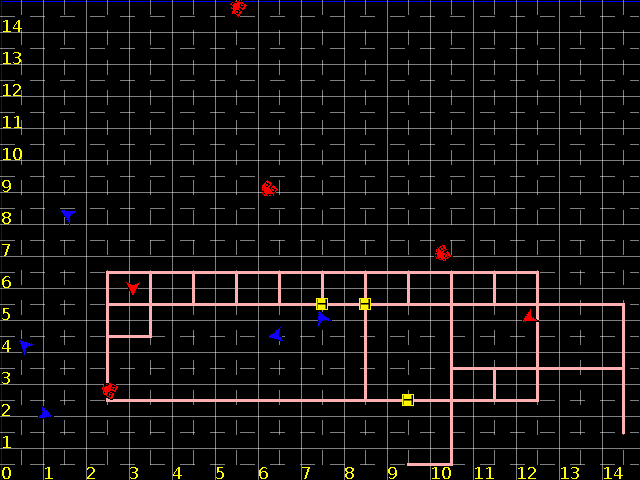
\includegraphics[scale=0.55]{world00.png}
	\caption{World 0}
	\label{fig:world0}
\end{figure}

\begin{figure}[H]
	\centering
	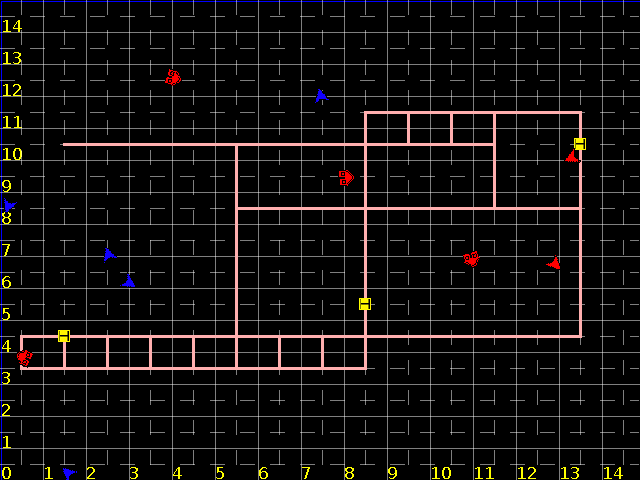
\includegraphics[scale=0.55]{world01.png}
	\caption{World 1}
	\label{fig:world1}
\end{figure}

\begin{figure}[H]
	\centering
	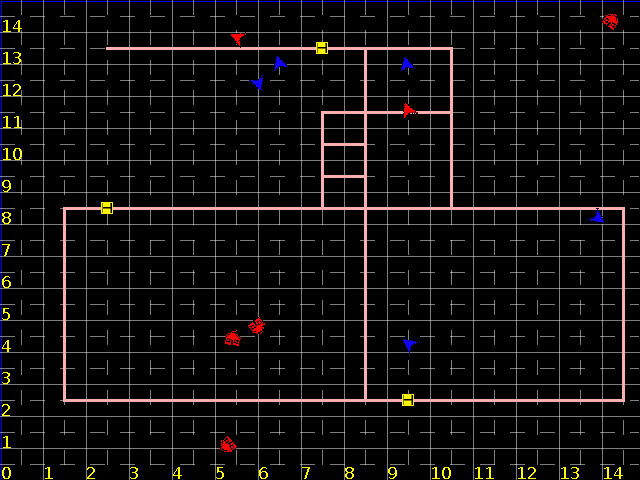
\includegraphics[scale=0.55]{world02.png}
	\caption{World 2}
	\label{fig:world2}
\end{figure}

\begin{figure}[H]
	\centering
	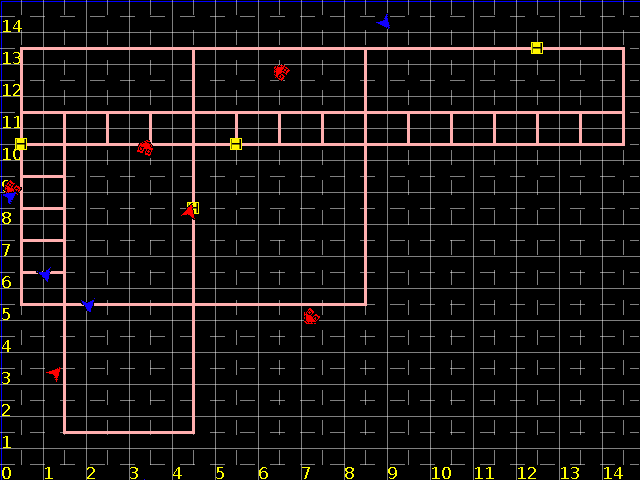
\includegraphics[scale=0.55]{world03.png}
	\caption{World 3}
	\label{fig:world3}
\end{figure}

\begin{figure}[H]
	\centering
	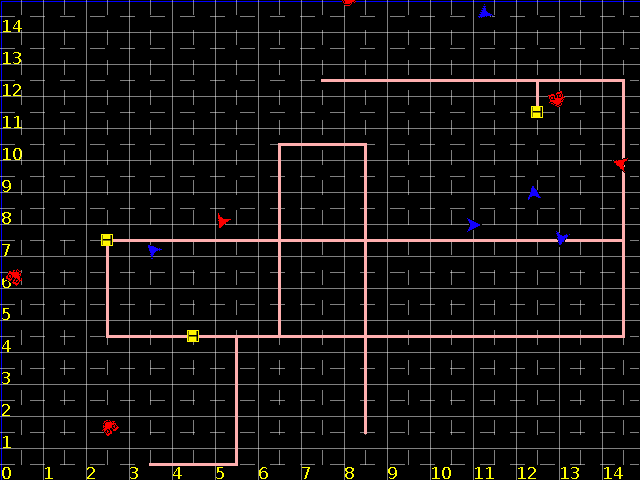
\includegraphics[scale=0.5]{world04.png}
	\caption{World 4}
	\label{fig:world4}
\end{figure}

\begin{figure}[H]
	\centering
	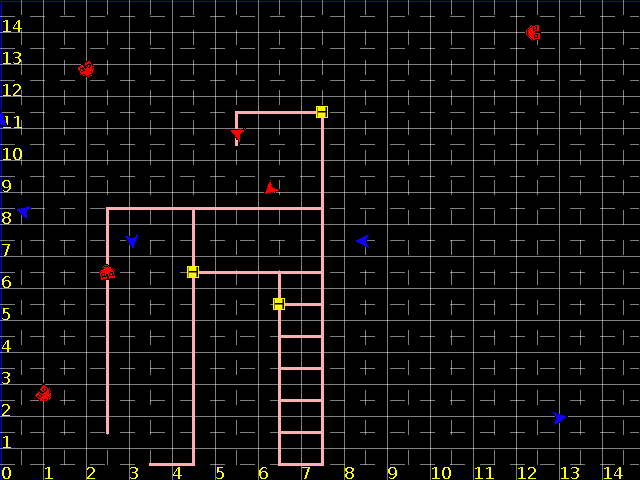
\includegraphics[scale=0.5]{world05.png}
	\caption{World 5}
	\label{fig:world5}
\end{figure}

\begin{figure}[H]
	\centering
	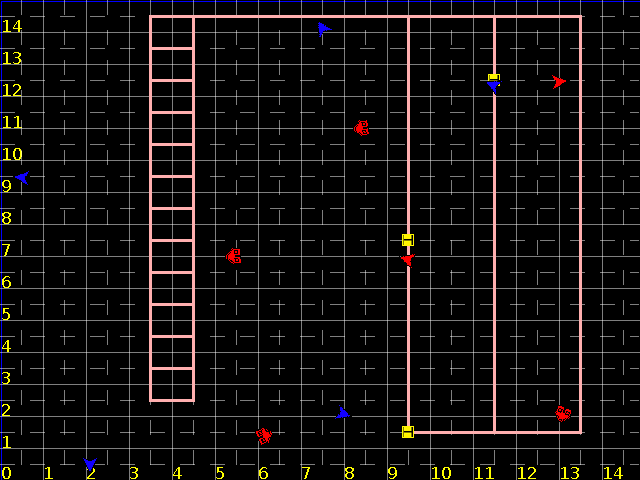
\includegraphics[scale=0.5]{world06.png}
	\caption{World 6}
	\label{fig:world6}
\end{figure}

\begin{figure}[H]
	\centering
	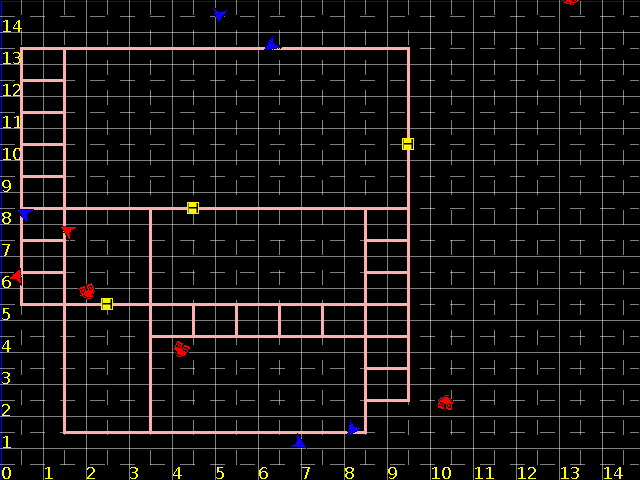
\includegraphics[scale=0.5]{world07.png}
	\caption{World 7}
	\label{fig:world7}
\end{figure}

\begin{figure}[H]
	\centering
	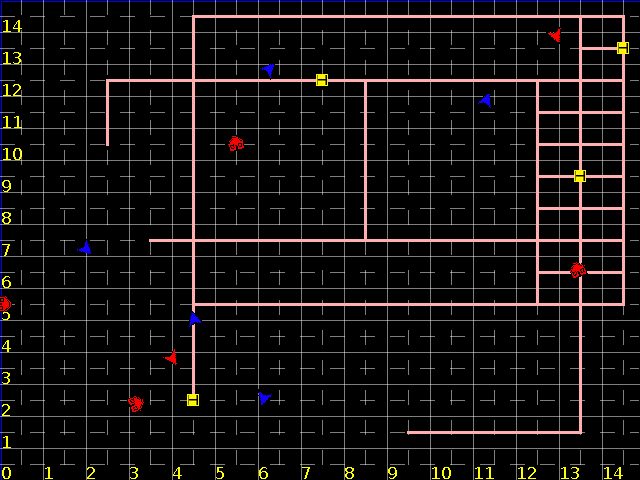
\includegraphics[scale=0.5]{world08.png}
	\caption{World 8}
	\label{fig:world8}
\end{figure}

\begin{figure}[H]
	\centering
	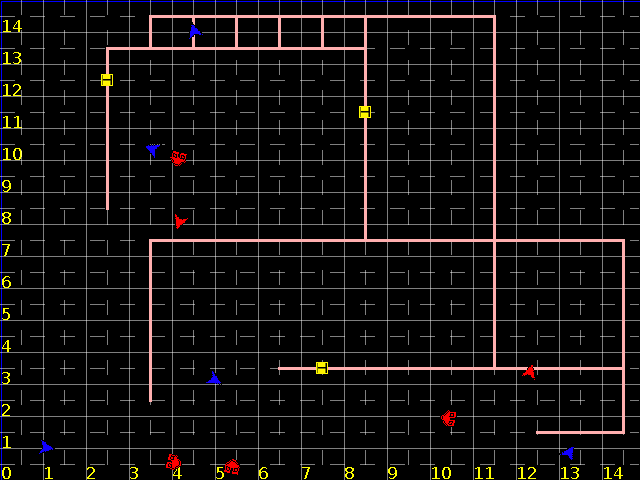
\includegraphics[scale=0.5]{world09.png}
	\caption{World 9}
	\label{fig:world9}
\end{figure}
